\section{PSR J0248$+$6021 and PSR J2240$+$5832: Characterizing Young Pulsars with RVM}
\paperref{This section is based on work done for
``PSRs J0248$+$6021 and J2240$+$5832: Young Pulsars in the Northern Galactic
Plane. Discovery, Timing, and $\gamma$-Ray Observations''
\citep{theureau2011psrs}. }


\begin{figure}[t!!]
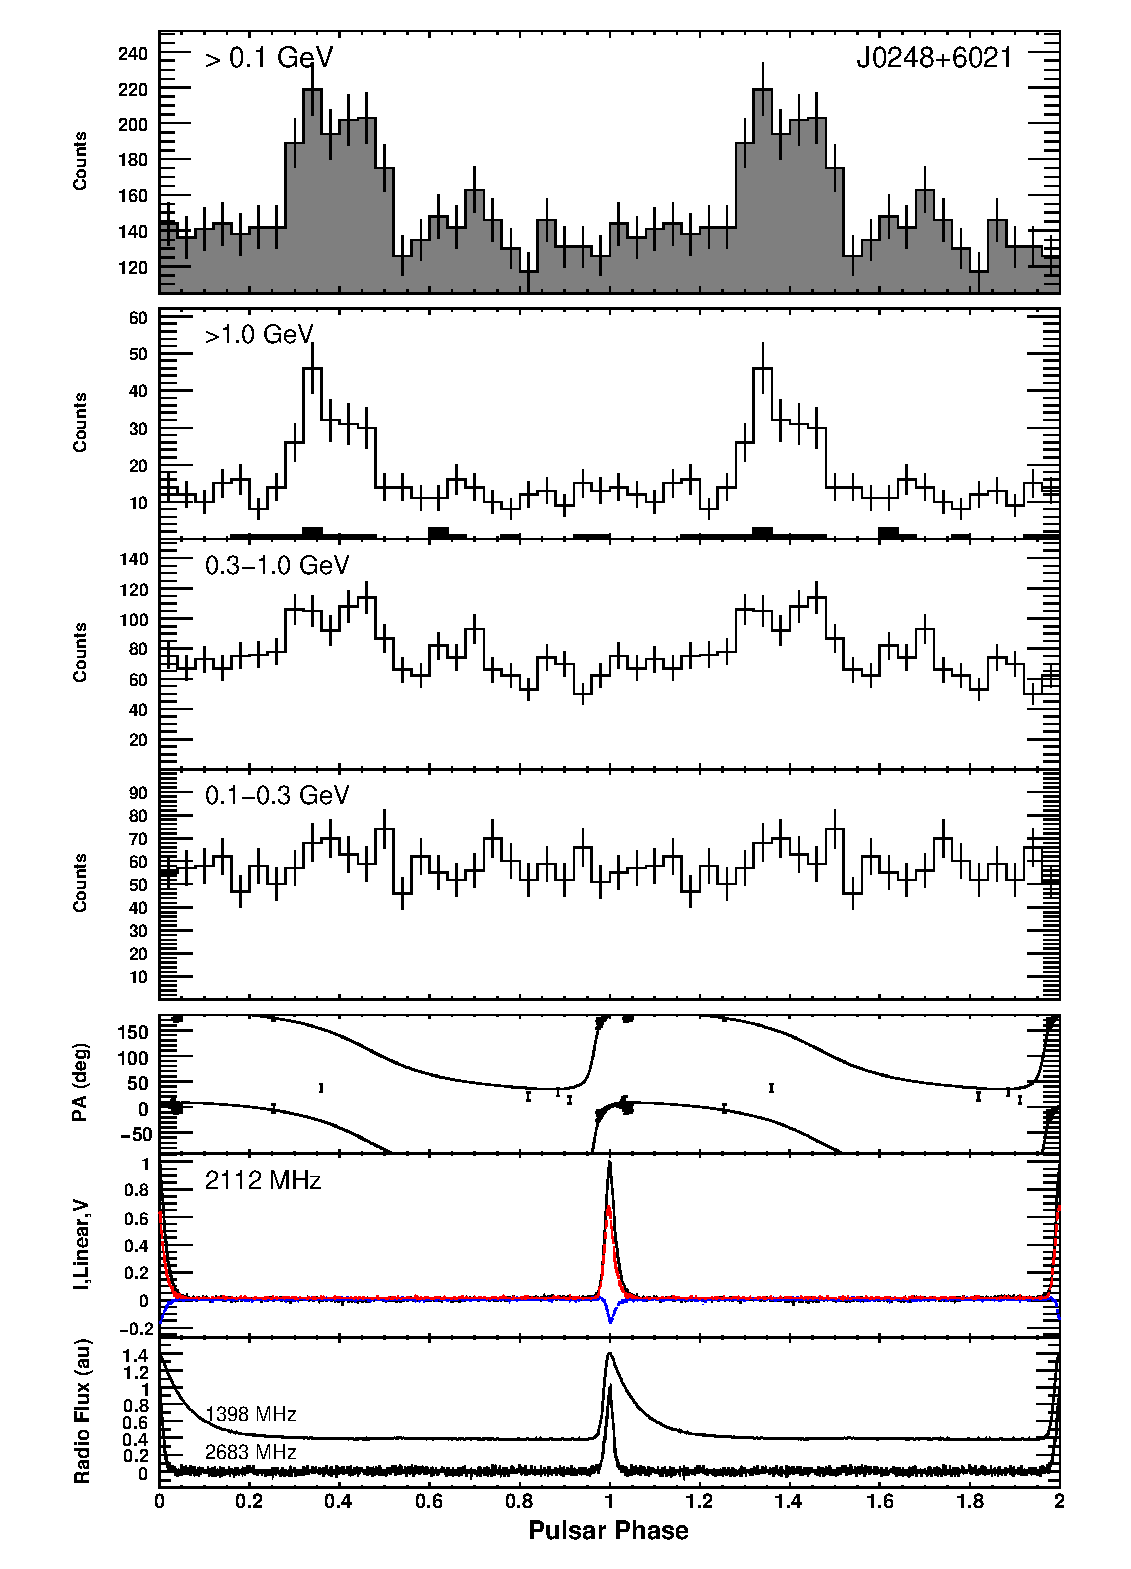
\includegraphics[width=0.5\textwidth]{chapters/multiWaveLength/figures/J0248+6021_catalog_lightcurve.eps}
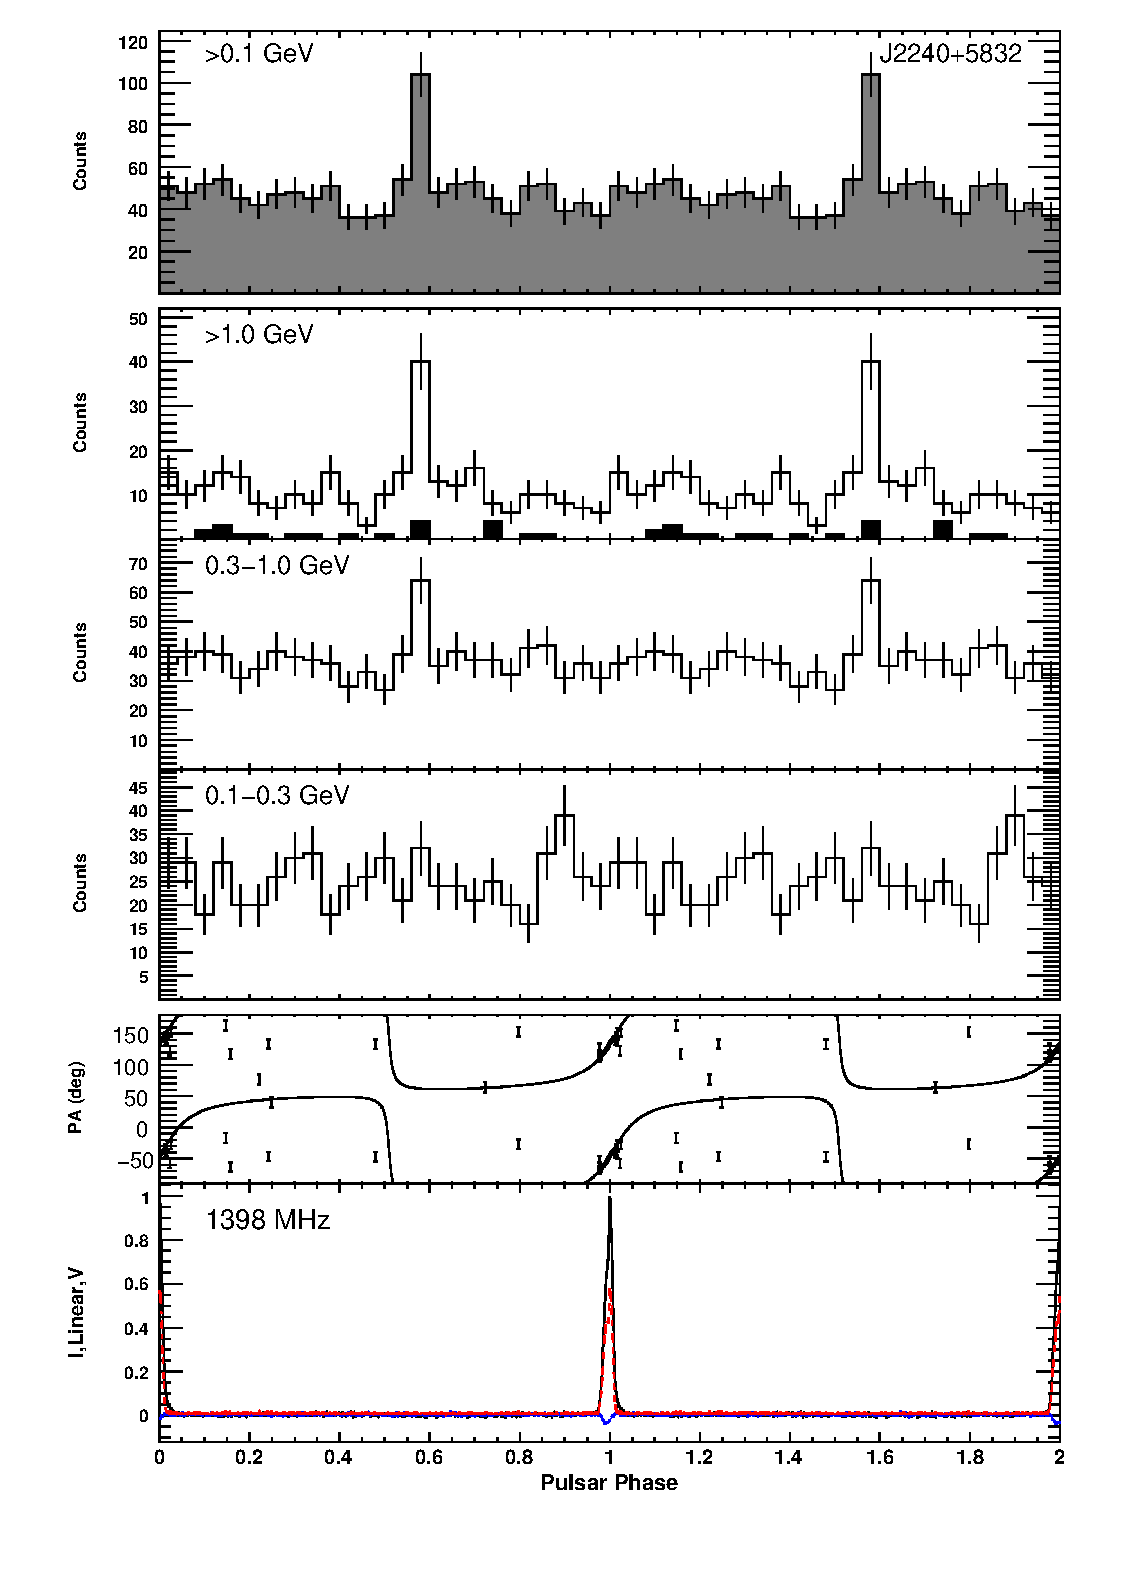
\includegraphics[width=0.5\textwidth]{chapters/multiWaveLength/figures/J2240+5832_catalog_lightcurve.eps}
\caption[Phase-aligned $\gamma$-ray and radio light curves for PSR J0248$+$6021 and PSR J2240$+$5832 obtained with
the \emph{Fermi} Large Area Telescope and the Nan\c cay Radio Telescope]{
Figure taken from \cite{theureau2011psrs}.
Phase-aligned $\gamma$-ray and radio light curves for PSR J0248$+$6021 and PSR J2240$+$5832 obtained with 
the \emph{Fermi} Large Area Telescope and the Nan\c cay Radio Telescope. 
The bottom panel for PSR J0248$+$6021 show the radio profiles at three frequencies. 
The second panel from the bottom
for PSR J0248$+$6021 and the bottom panel for PSR J2240$+$5832 
show the degree of linear (red dashed) and circular
polarizations (blue dotted), as well as the linear polarization position angle and a RVM fit.
The other panels show the
$\gamma$-ray light curve data in different energy bands. Two rotations are shown for clarity.}
\label{phasos}
\end{figure}

\begin{figure}[t!!]
\begin{center}
\includegraphics[width=0.8\textwidth]{chapters/multiWaveLength/figures/J0244Alpha46Zeta52Offset2.53133ANDJ2238Alpha108Zeta123Offsetneg45.818.ps}
\caption[Expanded view of the radio polarization position angle sweep near the peak in radio intensity]{Figure taken from \cite{theureau2011psrs}.
Expanded view of the radio polarization position angle sweep near the peak in radio intensity. 
The red points show the data used in the RVM fit. The black points failed the selection cuts
described in the text. Top two frames are data for PSR J2240$+$5832 at 1.4 GHz. The RVM curve shown corresponds to $\alpha = 108^\circ$ and $\zeta = 123^\circ$. Bottom two frames are data for PSR J0248+6021
at 2.1 GHz. The RVM curve shown corresponds to $\alpha = 46^\circ$ and $\zeta =52^\circ$.  \label{PolarZoom}
}
\end{center}
\end{figure}

\begin{figure}[t!!]
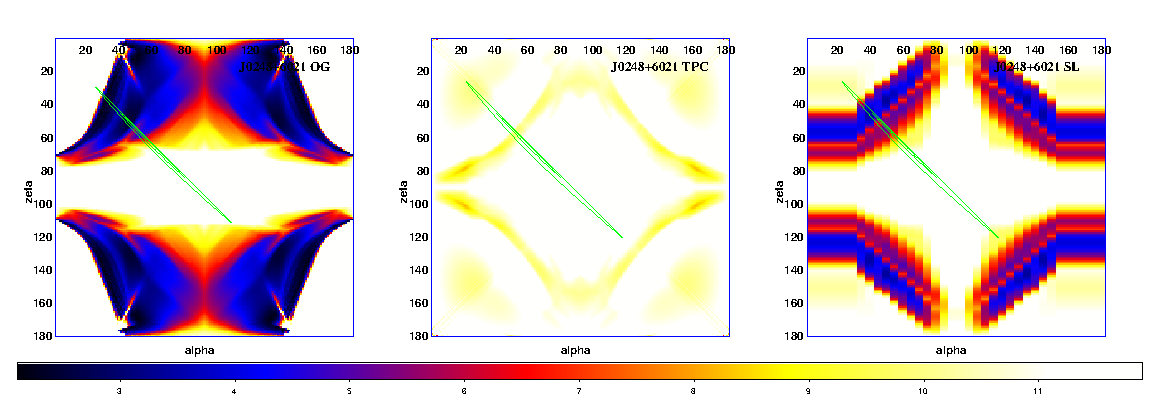
\includegraphics[width=1\textwidth]{chapters/multiWaveLength/figures/New_J0248_OGTPCSL.eps}
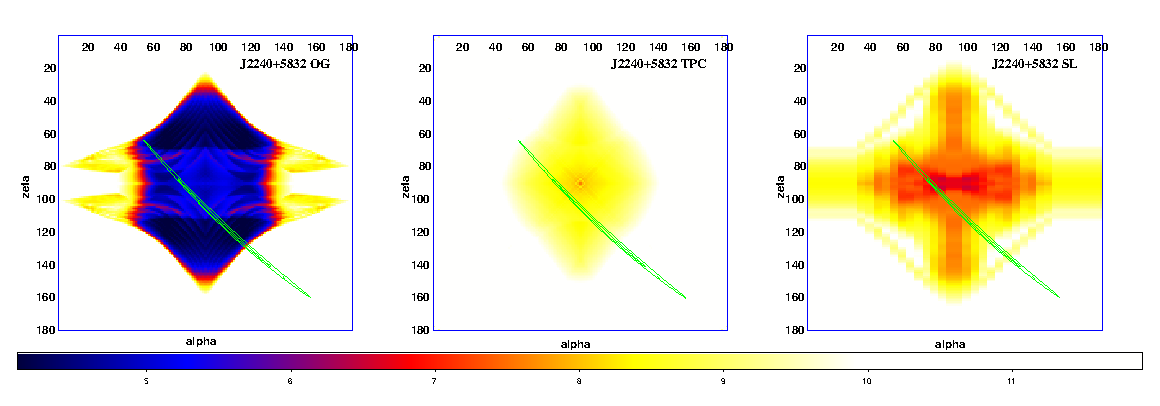
\includegraphics[width=1\textwidth]{chapters/multiWaveLength/figures/New_J2240_OGTPCSL.eps}
\caption[Pulsar geometry and emission modeling fit map for PSR J0248$+$6021 and PSR J2240$+$5832 in the $\alpha$--$\zeta$ plane]{Figure taken from \cite{theureau2011psrs}.
Pulsar geometry and emission modeling fit map for PSR J0248$+$6021 and PSR J2240$+$5832
in the $\alpha$--$\zeta$ plane. Green 
contours show the RVM fit to the radio polarization data. 
Contours are at $\delta(\chi^2/\text{Degree of Freedom}) = 0.25$ and $0.5$ above the minimum $\chi^2/\text{Degree of Freedom}$ of 1.6
for PSR J0248$+$6021 and $\delta(\chi^2/\text{Degree of Freedom}) = 0.4$ and $0.8$ above the minimum $\chi^2/\text{Degree of Freedom}$ of 5.1
for PSR J2240$+$5832.
The color backgrounds are $\chi_3$ maps of the fit to the observed $>100$\,MeV
pulse profile for the outer gap model (left),
the two-pole caustic model (middle), and the separatrix layer model (right), 
at different values of the magnetic inclination,
$\alpha$, and the minimum angle to the line-of-sight, $\zeta$ \citep{romani2010constraining}.
Each panel has the same color scale, where dark colors represent better fits. The
preferred models lie along the green RVM-selected band.
}
\label{OGTPC}
\end{figure}


PSR J0248$+$6021 ($P=217$ ms) and PSR J2240$+$5832 ($P=140$ms) are young pulsars first discovered in the radio
\citep{foster1997fast,ray1999j0248+}.  The polarization sweep for both pulsars is relatively smooth
such that likely only a single-altitude component contributes to the emission.

For these two pulsars, we applied both the RVM and $\gamma$-ray light curve models
to the available data.
Figure~\ref{phasos} shows the light curves at various wavelengths
as well as the polarization data.
Modeling results indicate that the $\gamma$-ray emission from PSR J0248$+$6021
is from a merged double $\gamma$-ray peak while the emission from 
PSR J2240$+$5832 is from a narrow caustic.
The paper discusses various measurements of the
pulsars PSR J0248$+$6021 and PSR J2240$+$5832 such as
flux density, proper motion, dispersion measure, kick velocity, and rotation
measure. 

We applied the RVM to the polarization data of 
PSR J0248$+$6021 (2.1 GHz) and PSR J2240$+$5832 (1.4 GHz).  
We cut on polarization with error bars greater than
 $\pm 2^\circ$.
The polarization position angle sweeps are flattened
due to scattering.  Data at 1.4 GHz was avaliable for PSR J0248$+$6021
but appeared distorted by scatter so only the 2.1 GHz data was used.
Red error bars on Figure~\ref{PolarZoom} show points
used in the fitting procedure.  

For PSR J0248$+$6021, the best fits give geometric angles $\beta\sim5^\circ$ 
(where $\beta=\zeta-\alpha$) and $\alpha$ between $25^\circ$ and $110^\circ$.
The best $\chi^2$ is 86.6 with reduced $\chi_{\rm{min}}^2=1.6$.
For PSR J2240$+$5832, the best fits give geometric angles $\beta\sim16^\circ$ and $\alpha$ between $75^\circ$ and $130^\circ$
although plausible solutions extended to $\alpha$ between $10^\circ$ and $150^\circ$.
The best $\chi^2$ is 86.6 with reduced $\chi_{\rm{min}}^2=1.6$.
Figure~\ref{PolarZoom} additionally shows reasonable model polarization sweeps
overlaid on data points.

On Figure~\ref{OGTPC}, green contours trace the best fit RVM in the $\alpha$-$\zeta$ plane.
The colored maps show best fit outer gap model, two-pole caustic model, 
and separatrix layer model \citep{bai2010modeling} to the $\gamma$-ray data.
The weighting used is the $\chi_3$ of \cite{romani2010constraining}.
For PSR J0248$+$6021, the best fit overlap between outer gap and RVM
model is $\alpha=46^\circ$ and $\zeta=52^\circ$.
For PSR J2240$+$5832, the best fit overlap between outer gap and RVM
models is $\alpha=101^\circ$ and $\zeta=117^\circ$.
Overall, the outer gap model seemed to be more consistent
with the polarization model results
than the other $\gamma$-ray models.



